\documentclass[a4paper,10pt]{article}
\usepackage[utf8]{inputenc}
\usepackage{amssymb}
\usepackage{graphicx}
\usepackage{hyperref}
\usepackage{algorithm,algpseudocode}
\usepackage{default}
\usepackage{xcolor}
\usepackage[francais]{babel}
\usepackage[top=3cm,bottom=3cm,right=3cm,left=3cm]{geometry}

\begin{document}

\author{LIMBALLE Pierre - PEREZ Quentin}
\title{Méthodes et Outils pour la Programmation\\% 
Mini Projet 2015}
\definecolor{primary}{RGB}{37,72,124}
\definecolor{secondary}{RGB}{253,250,200}

    
%\addtobeamertemplate{footline}{\insertframenumber/\inserttotalframenumber\\}
 %\addtobeamertemplate{sidebar bottom}{\insertframenumber}
\makeatletter
  \begin{titlepage}
  \centering
      {\LARGE \textbf{LIMBALLE Pierre - PEREZ Quentin}}\\
      UFR-ST - Licence informatique 3ème année\\Groupe TP 2B\\
    \vspace{2cm}
      {\LARGE \@date\\}
    \vspace{1cm}
        
\includegraphics[width=0.3\textwidth]{java.png}\\
    \vspace{1em}
       {\LARGE \textbf{\@title}\\
    \vspace{1em}
       Rapport\\} 
    \vspace{2em}
    \vspace{1cm}
        
\includegraphics[width=0.7\textwidth]{ufrst.jpg}\\
    \vspace{1.5cm}
      {Contacts : \href{mailto:pierre.limballe@edu.univ-fcomte.fr}{pierre.limballe@edu.univ-fcomte.fr}, \href{mailto:quentin.perez@edu.univ-fcomte.fr}{quentin.perez@edu.univ-fcomte.fr}\\Professeurs : GREFFIER Françoise, BONNEVILLE François}
    \vfill
        %\includegraphics[width=0.7\textwidth]{radare.png}\\
  \end{titlepage}
\makeatother

\newpage
\tableofcontents
\newpage

\section{Sujet}
\subsection{Contexte}
Dans le cadre du module: Méthodes et Outils pour la Programmation (MOP) la réalisation d'un projet nous a été demandé afin de mettre
en application les connaissances théoriques acquisent tout au long du semestre 5. \\
La conception de l'application a pour objectifs:
\begin{itemize}
  \item l'utilisation du langage de programmation Java en orienté objets
  \item l'application du paradigme MVC (Modèle - Vue - Contrôleur)
  \item l'approche du travail collaboratif par l'utilisation de logiciels de gestion de versions
  \item la manipulation d'éléments graphiques de la bibliothèque graphique Java Swing
\end{itemize}

\subsection{But de l'application}
La finalité de ce projet est la conception Java une application qui réalise une animation graphique en 2D 
représentant un ensemble de planètes et leurs satellites en orbite autour d'une ou plusieurs étoiles.
L'utilisateur doit disposer des fonctionnalités suivantes:
\begin{itemize}
  \item l'ajout et la suppression d'astres (étoiles ou satellites) dans l'application
  \item l'affichage des astres dans une fenetre graphique animée
  \item la possibilité de sauvegarder un système planétaire 
\end{itemize}
La contrainte d'ergonomie est également importante quant à l'utilisation du logiciel.

\newpage
\section{Conception}
\subsection{Introduction}
Planethacks est le nom choisi pour l'application. Du fait d'un travail en binôme, l'utilisation
d'un logiciel de gestion de version fut priviligiée. Nous avons pour cela utilisé Git, en lien avec le serveur d'hébergement \href{https://github.com}{GitHub} (sources GitHub de Planethacks: \url{https://github.com/qperez/planetacks}). 
\begin{center}
  $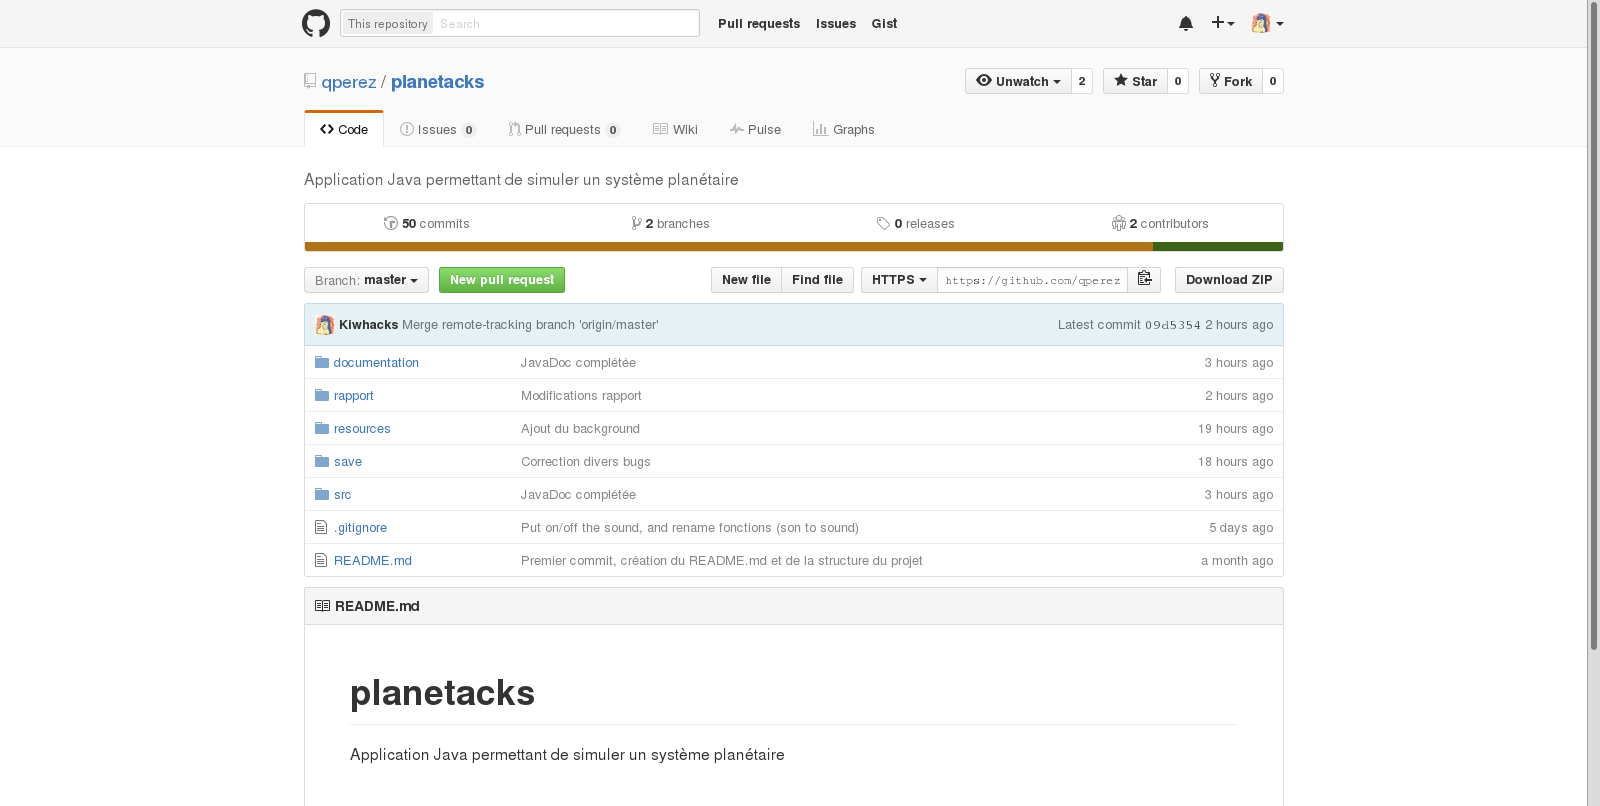
\includegraphics[scale=0.3]{git.png}$
\end{center}


L'IDE (\textit{Internal Development Environement}) IntelliJ IDEA fut utilisé durant toute la phase de développement et de tests et ce afin 
d'accélérer et faciliter le développement de l'application ainsi que son déboguage.\\
\begin{center}
  $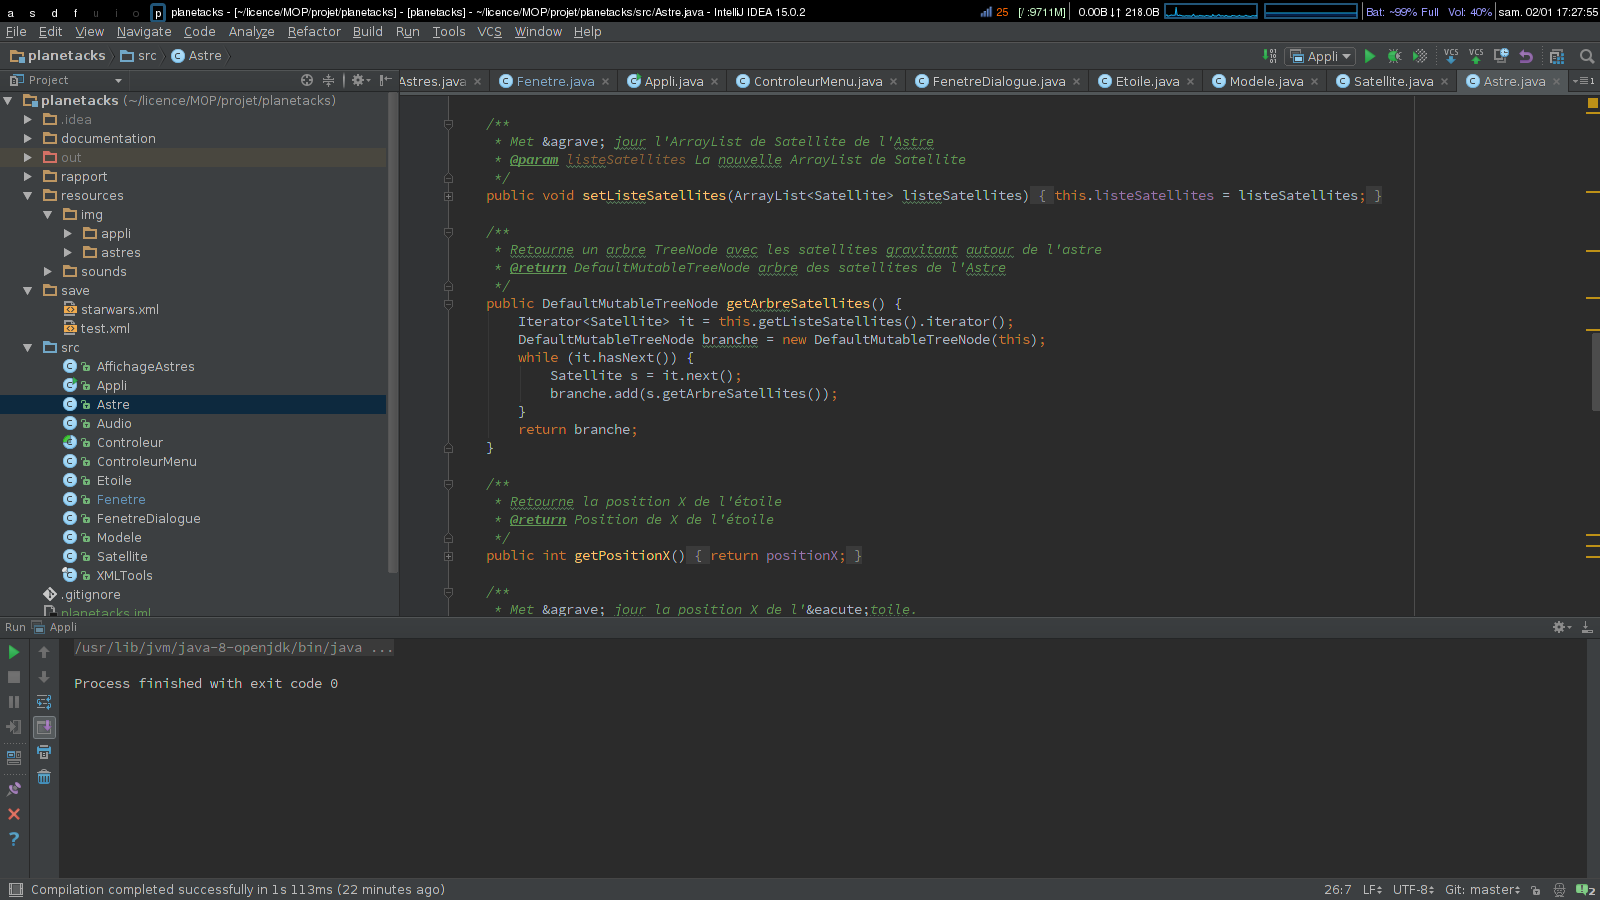
\includegraphics[scale=0.3]{idea.png}$
\end{center}

\subsection{Structures de données au sein de l'application}
La définition de classes permettant de structurer les données de notre programme fut la première étape de conception. Ainsi 3 classes 
nous permettent de modéliser un astre:
\begin{itemize}
  \item Astre (classe abstraite)
  \item Etoile
  \item Satellite
\end{itemize}

Planethacks repose sur une conception basée sur le paradigme MVC. Ce paradigme impose l'utilisation à minima de 3 classes (Modèle - Vue - Contrôleur) permettant de
séparer les données de l'affichage et des interactions utilisateur. \\ 
Dans un soucis de respect du modèle MVC nous disposons donc des classes suivantes:
\begin{itemize}
  \item Fenetre
  \item Modele
  \item Controleur (classe abstraite)
  \item ControleurMenu
  \item AffichageAstres
\end{itemize}

Afin de réaliser la fonctionnalité de sauvegarde une classe spécifique contenant les outils nécessaires fut créée: XMLTools. \\
Le point d'entré de l'application est assuré par la classe Appli.

\subsubsection{Modélisation d'un astre (Etoile ou Satellite)}
Le diagramme UML ci-dessous représente la modélisation choisie pour un astre:
\begin{center}
  $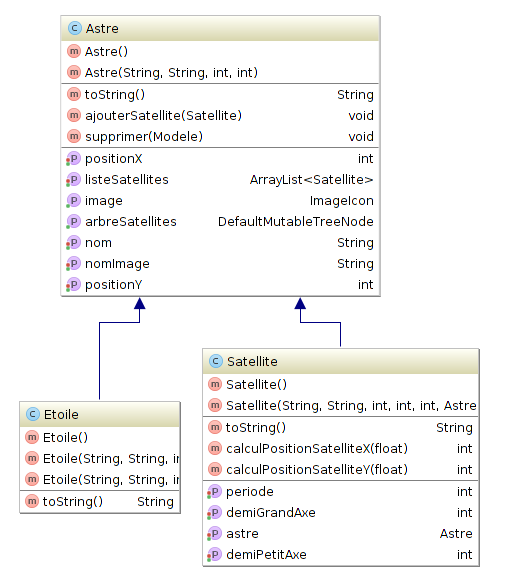
\includegraphics[scale=0.4]{classes_astre.png}$
\end{center}
Les méthodes \textit{calculPositionSatelliteX(float)} et \textit{calculPositionSatelliteX(float)} présentes dans la classe Satellite permettent
de calculer la position en X et en Y du Satellite en fonction du temps. La méthode \textit{ajouterSatellite(Satellite)} permet de mettre en orbite un satellite autour d'un astre. Enfin, la méthode \textit{supprimer(Modele)} permet de supprimer récursivement un astre et ses satellites à partir du modèle donné.

\subsection{Structure générale de l'application}

\subsubsection{Emplacement des fichiers}
Nous avons utilisé une structure de fichiers qui nous parraissait être la plus simple et la meilleure pour le fonctionnement de l'application. Ci-dessous, une représentation de l'arborescence :\\
\begin{center}
  $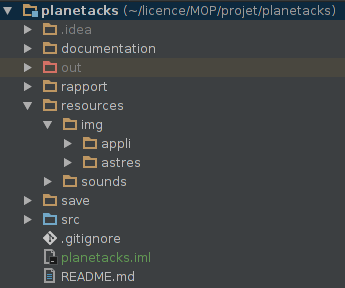
\includegraphics[scale=0.7]{arbo.png}$
\end{center}

Nous pouvons retrouver les dossiers de production suivants, dans lesquels nous manipulions directement les fichiers :
\begin{itemize}
 \item \begin{verbatim}src\end{verbatim} $\rightarrow$ dossier des sources (.java)
 \item \begin{verbatim}ressources\end{verbatim} $\rightarrow$ dossier des différents fichiers image ou audio
 \begin{itemize}
  \item \begin{verbatim}img\end{verbatim} $\rightarrow$ dossier contenant toutes les images du projet
  \begin{itemize}
   \item \begin{verbatim}appli\end{verbatim} $\rightarrow$ dossier des images de l'application en général
   \item \begin{verbatim}astres\end{verbatim} $\rightarrow$ dossier des images des astres (.png)
  \end{itemize}
  \item \begin{verbatim}sounds\end{verbatim} $\rightarrow$ dossier contenant tous les sons du projet
 \end{itemize}
 \item \begin{verbatim}rapport\end{verbatim} $\rightarrow$ dossier contenant les fichiers permettant de réaliser ce rapport (fichiers \LaTeX)
\end{itemize}
\vspace{0.5cm}
Mais également des dossiers dont le contenu est généré automatiquement :
\begin{itemize}
 \item \begin{verbatim}out\end{verbatim} $\rightarrow$ dossier des fichiers java compilés (.class)
 \item \begin{verbatim}save\end{verbatim} $\rightarrow$ dossier des fichiers de sauvegarde générés par l'application (.xml)
 \item \begin{verbatim}documentation\end{verbatim} $\rightarrow$ dossier contenant la documentation du projet (.html)
 \item \begin{verbatim}.idea\end{verbatim} $\rightarrow$ dossier contenant les fichiers de configuration du logiciel \textit{IntelliJ IDEA}
\end{itemize}
\vspace{0.5cm}
Ainsi que des fichiers seuls :
\begin{itemize}
 \item \begin{verbatim}.gitignore\end{verbatim} $\rightarrow$ fichier permettant d'ignorer l'envoi de fichiers sur GitHub (ex : dossier \textit{out})
 \item \begin{verbatim}README.md\end{verbatim} $\rightarrow$ fichier MarkDown de présentation du projet sur GitHub
 \item \begin{verbatim}planetacks.iml\end{verbatim} $\rightarrow$ fichier de configuration du projet pour \textit{IntelliJ IDEA}
\end{itemize}

\subsubsection{Architecture MVC}
\begin{center}
  $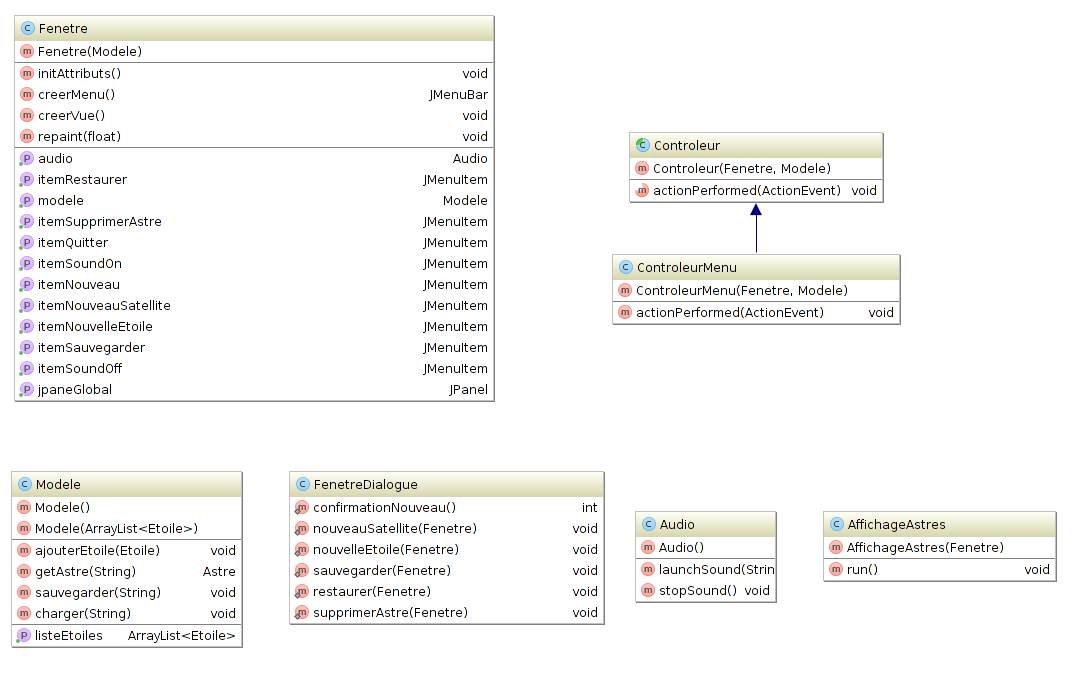
\includegraphics[scale=0.4]{classes_mvc.png}$
\end{center}


\subsection{Les algorithmes intéressants}

\begin{algorithm}
\caption{méthode repaint de la classe Fenetre}
\begin{algorithmic}
\Function{repaint}{t temps}
\State Supprimer l'ensemble des composants graphique du JPanel
\For{chaque Etoile $e$ de la liste d'étoiles du Modele}
    \State $jlabastre\gets$ nouveau JLabel avec l'image de $e$
    \State Afficher $jlabastre$ en fonction de la position $X_{e}$ et $Y_{e}$
    \State Ajouter le $jlabastre$ au JPanel
    \For{chaque Satellite $s$ de la liste des satellites de $e$}
	\State $jlabsat\gets$ nouveau JLabel avec l'image de $s$
	\State Afficher $jlabsat$ en fonction de $s.calculPositionSatelliteX(t)$ et $s.calculPositionSatelliteY(t)$
	\State Ajouter le $jlabsat$ au JPanel
    \EndFor
\EndFor
\State Appel de la méthode $repaint()$ sur le JPanel
\EndFunction
\end{algorithmic}
\end{algorithm}

\subsection{Points intéressants et supplémentaires du programme}

\newpage
\section{Conclusion}
\subsection{Bilan}

\subsection{Les acquis}

\subsection{Améliorations futures}

\end{document}
